%
% $Id: $
%
%
% Compilar a .pdf con LaTeX (pdflatex)
% Es necesario instalar Beamer (paquete latex-beamer en Debian)
%

%
% Gr�ficos:
% Los gr�ficos pueden suministrarse en PNG, JPG, TIF, PDF, MPS
% Los EPS deben convertirse a PDF (usar epstopdf)
%

\documentclass{beamer}
\usetheme{Warsaw}
%\usebackgroundtemplate{
\includegraphics[width=\paperwidth]{format/libresoft-bg.png}}
%\usepackage[spanish]{babel}
\usepackage[latin1]{inputenc}
\usepackage{graphics}
\usepackage{amssymb} % Simbolos matematicos
\usepackage{url}
\usepackage{multirow}


%\definecolor{libresoftgreen}{RGB}{162,190,43}
%\definecolor{libresoftblue}{RGB}{0,98,143}

%\setbeamercolor{titlelike}{bg=libresoftgreen}

%% Metadatos del PDF.
\hypersetup{
  pdftitle={Code to learn with Scratch? A systematic literature review},
  pdfauthor={J. Moreno-Le�n, Gregorio Robles},
  pdfcreator={GSyC/LibreSoft \\ Universidad Rey Juan Carlos},
  pdfproducer=PDFLaTeX,
  pdfsubject={Code to learn with Scratch},
}
%%

\begin{document}

\title{Code to learn with Scratch?}
\subtitle{A systematic literature review}
\institute{jesus.moreno@programamos.es, grex@gsyc.urjc.es \\
GSyC/Libresoft, Universidad Rey Juan Carlos}
\author{J. Moreno-Le�n, Gregorio Robles}
\date{IEEE EDUCON 2016, Abu Dhabi, April 12\textsuperscript{th} 2016}

\frame{
\maketitle
\begin{center}

\includegraphics[width=2cm]{format/libresoft-logo}
\hspace{0.5cm}

\includegraphics[width=5cm]{format/gsyc-urjc}
\vspace{0.5cm}

\includegraphics[width=3cm]{format/emadrid.png}
\end{center}
}


% Si el titulo o el autor se quieren acortar para los pies de p�gina
% se pueden redefinir aqu�:
%\title{Titulo corto}
%\author{Autores abreviado}

%% LICENCIA DE REDISTRIBUCION DE LAS TRANSPAS
\frame{
~
\vspace{3cm}

\begin{flushright}

\includegraphics[width=2.2cm]{figs/by-sa}

{\tiny
(cc) 2016 J. Moreno-Le�n and Gregorio Robles\\
  Some rights reserved. This work licensed under Creative Commons \\
  Attribution-ShareAlike License. To view a copy of full license, see \\
  http://creativecommons.org/licenses/by-sa/3.0/ or write to \\
  Creative Commons, 559 Nathan Abbott Way, Stanford, \\
  California 94305, USA. \\
\ \\
Some of the figures have been taken from the Internet \\
Source, and author and licence if known, is specified. \\
For those images, \emph{fair use} applies.
}
\end{flushright}
}
%%

\section{EDUCON 2016, Abu Dhabi}


%--------------------------------------------------------
%\usebackgroundtemplate{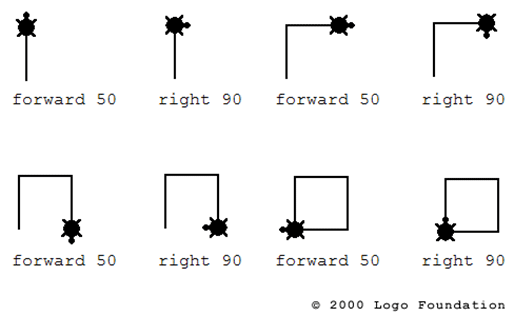
\includegraphics[height=10cm]{figs/turtles.png}}
% background: http://www.wim-network.org/wp-content/uploads/2012/04/iceberg.jpg

\begin{frame}
\frametitle{Code to learn (I)}
\begin{columns}[T]
  \begin{column}{0.5\textwidth}
    \begin{figure}[t!]
      \begin{center}
	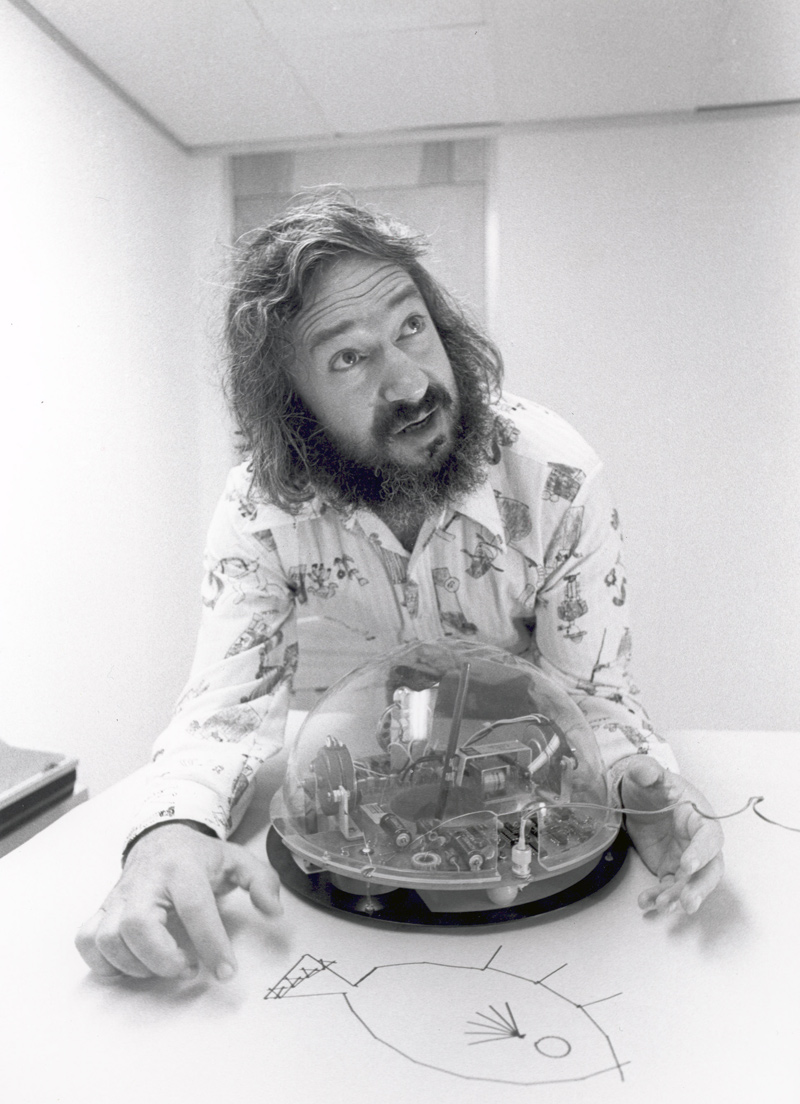
\includegraphics[width=5cm]{figs/seymour.jpg}
      \end{center}
      \label{fig:repetition1}
    \end{figure}
  \end{column}
  \begin{column}{0.5\textwidth}
    \begin{block}{Logo programming language}
      \begin{itemize}
	 \item Developed in the 1960s
         \item Its educational impact was intensively investigated in the 70s and 80s
         \item Students' improvements in maths (and other disciplines) were proved
         \item ``Disappeared'' from the educational landscape since mid-90s
      \end{itemize}
    \end{block}
    \hfill{\Tiny Seymour Papert's picture: jgora.net}
  \end{column}
\end{columns}
\end{frame}

\usebackgroundtemplate{}
%--------------------------------------------------------
\usebackgroundtemplate{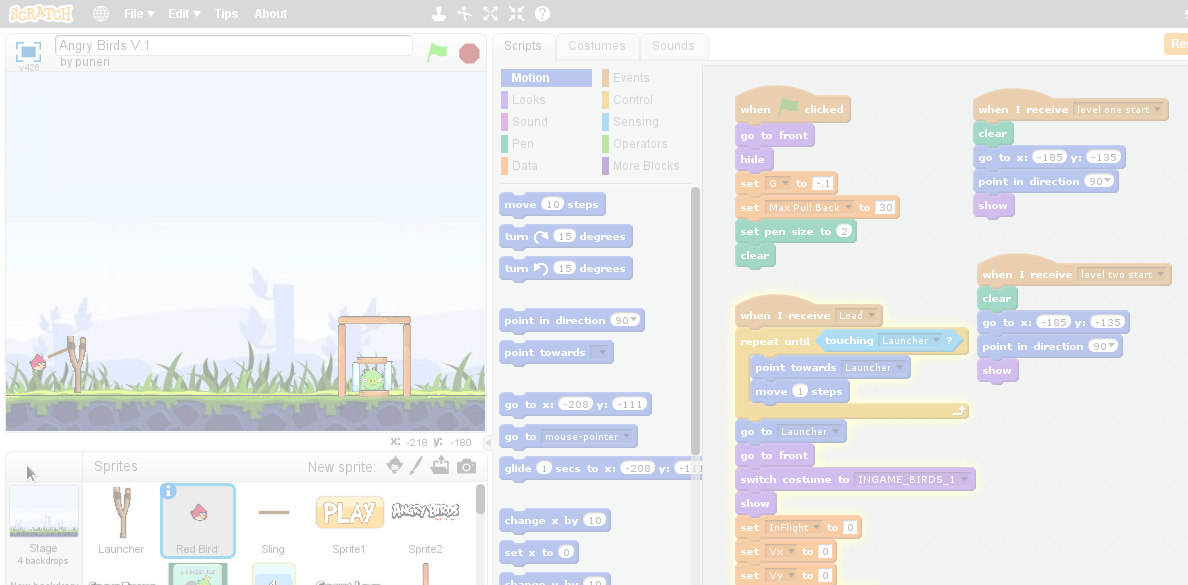
\includegraphics[width=18cm]{figs/AngryBirds2.png}}
\begin{frame}
\frametitle{Code to learn (and II)}

\begin{columns}[T]
  \begin{column}{1\textwidth}
     \begin{block}{New visual programming languages}
       \begin{itemize}
	 	 \item Alice, Greenfoot, Kodu, \textbf{Scratch}
         \item Code.org, EU Code Week, Africa Code Week, ArabCode.org 
         \item If there is no evidence showing educational impact of programming, this resurgence of programming in schools could disappear in a few years.
       \end{itemize}
    \end{block}
  \end{column}
\end{columns}

\end{frame}
\usebackgroundtemplate{}
%--------------------------------------------------------
\usebackgroundtemplate{
\includegraphics[width=14cm]{figs/goals.jpg}}
%https://rebel-performance.com/wp-content/uploads/2014/10/goals.jpg

\begin{frame}
\frametitle{Research questions}

\begin{itemize}
\item \Large  {\bf RQ1. What K-12 subjects have used programming with Scratch as an educational resource?}\\
\item \Large  {\bf RQ2. Is programming with Scratch a good educational tool that enhances student learning?}\\
\item \Large  {\bf RQ3. What other skills are developed while learning to code with Scratch?}
\end{itemize}
\hfill{\Tiny Background picture: rebel-performance.com}
\end{frame}

\usebackgroundtemplate{}
%-----------------------    ---------------------------------

\begin{frame}
\frametitle{Methodology}
\begin{center}
	\begin{figure}[t!]
		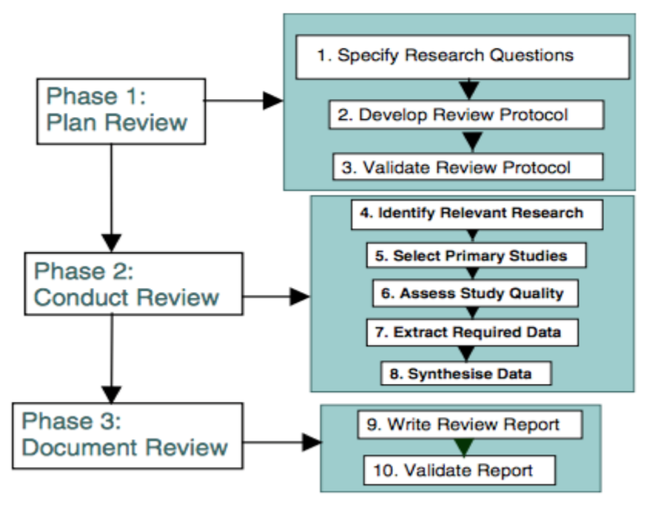
\includegraphics[width=7cm]{figs/slr.png}    
    		\caption{Systematic literature review process}
	\end{figure}
	\tiny Source: \textit{Guidelines for Performing Systematic Literature Reviews in Software Engineering}
\end{center}

\end{frame}

\usebackgroundtemplate{}

%%--------------------------------------------------------


\begin{frame}
\frametitle{Selection of primary studies}
Out of 107 located articles, the final number of selected papers is 15.
\begin{table}
\begin{center}
  \begin{tabular}{ | l | c | }
   \hline
    \multicolumn{1}{|c|}{\textbf{Motive of exclusion}} & \multicolumn{1}{c|}{\textbf{Number of papers}} \\ \hline\hline
    Focused on programming & 32 \\ \hline
    No evidence provided & 7 \\ \hline
    University students & 7 \\ \hline
    Out of context & 41 \\ \hline
    No English version & 2 \\ \hline
    Articles not accessed & 3 \\ \hline
  \end{tabular}
\end{center}
\caption{Summary of article exclusion}
\end{table}
\end{frame}


%-----------------------    ---------------------------------

\begin{frame}
\frametitle{Findings, RQ1}
\begin{table}
\small
\begin{center}
  \begin{tabular}{ | c | c | c | c | }
   \hline
    \multicolumn{1}{|c|}{\textbf{Paper}} & \multicolumn{1}{c|}{\textbf{Age}} & \multicolumn{1}{c|}{\textbf{Subject}} & \multicolumn{1}{c|}{\textbf{Environment}} \\ \hline\hline
    [21] & Middle School & Mathematics & School  \\ \hline
    [22] & 5th grade & Mathematics, Language Arts & Summer camp \\ \hline
    [23] & 3rd grade & Mathematics & School \\ \hline
    [24] & 5th grade & Science & School \\ \hline
    [25] & 5th grade & Science & School \\ \hline
    [26] & 10-14 years old & Storytelling, Creative writing & After school \\ \hline
    [27] & 12-14 years old & Writing & School \\ \hline
    [28] & 4th-5th grade & English as a second language & School\\ \hline
  \end{tabular}
\end{center}
\caption{Subjects learned through coding with Scratch}
\end{table}

\end{frame}

\usebackgroundtemplate{}

%-----------------------    ---------------------------------

\begin{frame}
\frametitle{Findings, RQ2}
\begin{center}
	\begin{figure}[t!]
		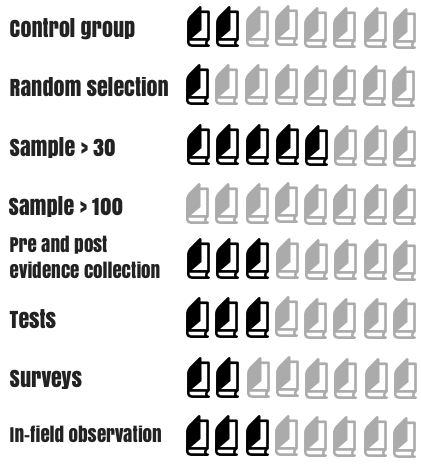
\includegraphics[width=5.5cm]{figs/rq2_description.png}    
    		\caption{Description of the 8 papers under investigation for RQ2}
	\end{figure}
\end{center}

\end{frame}


\usebackgroundtemplate{}

%-----------------------    ---------------------------------

\begin{frame}
\frametitle{Findings, RQ2}
\begin{table}[]
\scriptsize
\centering
\begin{tabular}{|c|c|p{4.4cm}|p{3.8cm}|}
\hline
\multicolumn{1}{|c|}{\textbf{Subject}} & \multicolumn{1}{|c|}{\textbf{Paper}} & \multicolumn{1}{|c|}{\textbf{Proved results}} & \multicolumn{1}{|c|}{\textbf{Non-proved results}} \\ \hline\hline
\multirow{3}{*}{Maths} & [21] & Significantly more positive attitudes towards maths &  \\ \cline{2-4} 
                  & [22] & Test scores in maths highly correlated with programming performance &  \\ \cline{2-4} 
                  & [23] & Improvements at comparing numbers and establishing order & No differences at spatial location \\ \hline
\multirow{2}{*}{Science} & [24] &  & How or if learners deepened their science knowledge \\ \cline{2-4} 
                  & [25] & 61.5\% reported a better understanding of science &  \\ \hline
\multirow{2}{*}{L. arts} & [26] & 60\% indicated their storytelling skills improved &  \\ \cline{2-4} 
                  & [27] & Effective framework for facilitating digital composition &  \\ \hline
English & [28] & Experimental improved more than control groups &  \\ \hline
\end{tabular}
\caption{Programming with Scratch to learn other subjects}
\end{table}
\end{frame}

\usebackgroundtemplate{}

%-----------------------    ---------------------------------

\begin{frame}
\frametitle{Findings, RQ3}
\begin{center}
	\begin{figure}[t!]
		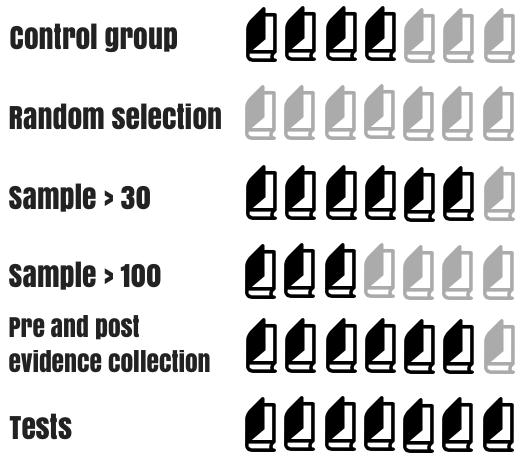
\includegraphics[width=5.5cm]{figs/rq3_description.png}    
    		\caption{Description of the 7 papers under investigation for RQ3}
	\end{figure}
\end{center}

\end{frame}


\usebackgroundtemplate{}

%-----------------------    ---------------------------------

\begin{frame}
\frametitle{Findings, RQ2}
\begin{table}[]
\scriptsize
\centering
\begin{tabular}{|c|p{4.4cm}|p{3.8cm}|}
\hline
\multicolumn{1}{|c|}{\textbf{Paper}} & \multicolumn{1}{|c|}{\textbf{Proved results}} & \multicolumn{1}{|c|}{\textbf{Non-proved results}} \\ \hline\hline
[25] & Better performance in logical thinking and problem solving &  \\ \hline
[30] & Students in the treatment group show improvement in their problem solving skills at a rate greater than those in the control group &  \\  \hline
[31] & Improved problem solving ability &  \\ \hline
[32] & The effect on problem solving abilities is significant, especially at the reason of prediction &  No significant effect on logical reasoning skills \\  \hline
[33] & Improved problem solving skills and reasoning practices &  \\ \hline
[34] & Increase in self-confidence in problem solving ability & No significant differences in problem solving skills \\  \hline
[35] & Increase in logic, creativity and learning skills &  \\ \hline
\end{tabular}
\caption{Skills developed by programming with Scratch}
\end{table}
\end{frame}

\usebackgroundtemplate{}

%-----------------------    ---------------------------------
\usebackgroundtemplate{
\includegraphics[width=13cm]{figs/take-away.jpg}}
%% background: http://flamingcow.co.uk/wp-content/uploads/2015/02/takeaway-940x283.jpg
\begin{frame}
\frametitle{Conclusions}
\hfill{\Tiny background picture: http://flamingcow.co.uk}
\end{frame}

\usebackgroundtemplate{}


%%--------------------------------------------------------

\usebackgroundtemplate{
\includegraphics[width=13cm]{figs/future.png}}

\begin{frame}
\frametitle{Future Work}

%\begin{enumerate}
%  \item Increase the number of students
%  \item Increase the type of subjects 
%  \item Increase the working time of programming
%\end{enumerate}
%\vspace{\baselineskip}
%\vspace{\baselineskip}
\hfill{\Tiny Background picture: Simon Cunningham }
%
\end{frame}
%
%%--------------------------------------------------------
%%\begin{frame}
%%\frametitle{GSyC/LibreSoft}
%
%%\begin{figure}[t!]
%%\begin{center}
%%\includegraphics[width=11cm]{figs/libresoft.jpg}
%%\end{center}
%%\label{fig:libresoft}
%%\end{figure}
%
%%\begin{center}
%%The GSyC/LibreSoft research team at URJC (Madrid).
%%\end{center}
%
%%\end{frame}
%
%%--------------------------------------------------------
%%\begin{frame}
%%\frametitle{Our work at GSyC/LibreSoft}
%
%%\begin{figure}[t!]
%%\begin{center}
%%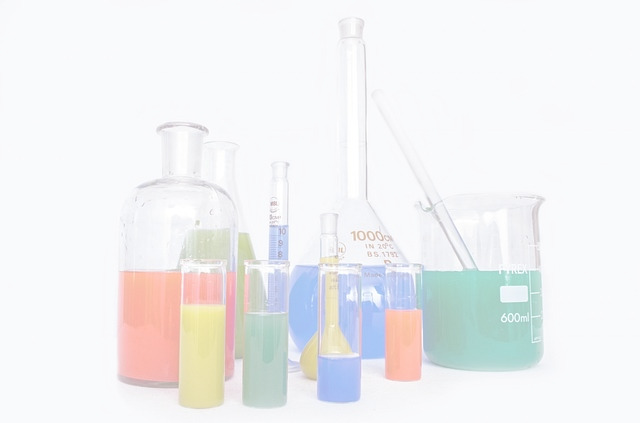
\includegraphics[width=2.5cm]{figs/research}
%% http://www.memphis.edu/crow/images/research_2.jpg
%%\hspace{0.1cm}
%%\includegraphics[width=2.5cm]{figs/teaching}
%% http://2.bp.blogspot.com/_uxgwfriLwSo/TOWDr8IjaLI/AAAAAAAABLM/d7H-G5jIq-c/s1600/teaching.gif
%%\hspace{0.1cm}
%%\includegraphics[width=2.5cm]{figs/development}
%% http://www.vidadigitalradio.com/wp-content/uploads/2009/04/hackers_cartoons.jpg
%%\hspace{0.1cm}
%%\includegraphics[width=2.5cm]{figs/promotion}
%% http://bloggeate.com/wp-content/uploads/2011/04/como-promocionar-tu-blog.jpg
%%\end{center}
%%\label{fig:whatwedo}
%%\end{figure}
%
%%\begin{center}
%%GSyC/LibreSoft's tasks: research, teaching, development, promotion of free software.
%
%%\end{center}
%%\end{frame}
%
\usebackgroundtemplate{}

%--------------------------------------------------------
\frame{
\maketitle
\begin{center}

\includegraphics[width=2cm]{format/libresoft-logo}
\hspace{0.5cm}

\includegraphics[width=5cm]{format/gsyc-urjc}
\vspace{0.5cm}

\includegraphics[width=3cm]{format/emadrid.png}
\end{center}
}

\end{document}
